\documentclass{article}
\usepackage{amsmath}
\usepackage{mathrsfs}
\usepackage{amssymb}
\usepackage{amsfonts}
\usepackage{gauss}
\usepackage[top=1in,bottom=1in,left=1.25in,right=1.25in]{geometry}
\usepackage{dsfont}
\usepackage{amsthm}
\usepackage{graphicx}
\usepackage{multirow}
\usepackage{textcomp}
\usepackage{bbm}
\usepackage{wasysym}
\usepackage{fancyhdr}
\pagestyle{fancy}
\lhead{Instructor: Prof. Krzyzosiak}
\chead{VP160 Project}
\rhead{SJTU-UM Joint Institude}
\lfoot{}
\cfoot{\thepage}
\rfoot{}

\begin{document}
\section{Introduction}
$\indent$To solve the equation of motion of a particle according to Newton’s Law, there are two different methods to find approximate solution for the equation:
$$\frac{d^2\mathbf{r}}{dt^2}=\frac{F(\mathbf{v},\mathbf{r},t)}{m}$$
$\indent$The first method is the Euler method, which use the slope of function $f$ at the beginning point to product a straight line from the beginning point with $x$-coordinate $(t)$ to the end point with $x$-coordinate $(t+\Delta t)$. Do this step more and get an appoximate figure of function $f$. The essence of the Euler method is a Taylor expansion of function $f$ at instant of time $t+\Delta t$ and neglect terms of order higher than one in $\Delta t$.\\
$\indent$Another method is the Second-order Runge-Kutta method, which use the slope of function $f$ at the beginning point to product a straight line from the beginning point with $x$-coordinate $(t)$ to the end point with $x$-coordinate $(t+\Delta t)$. Then take the half of the $y$-coordinate of the end point and find the slope of the point on the function $f$ with the same $y$-coordinate as the slope of the new straight line from the beginning poing to a new end point. Do the step more and get an appoximate figure of function $f$. The essence of the Second-order Runge-Kutta method is a Taylor expansion of function $f$ at instant of time $t+\Delta t$ and neglect terms of order higher than two in $\Delta t$.\\
$\indent$To identify how these two method work, we are going to approximately solve two problems: Projectile motion with air drag and Simple harmonic oscillator. By comparing the approximate solutions, whether the methods are efficient under some situation can be found.
\\\indent Almost all the algorithms and plots are implemented by MATLAB on WIN7, and only one program is run by Mathematica.
\section{Projectile motion with air drag}
We use MATLAB to finish plotting of this part.
\subsection{}
According to Euler Method:
\begin{eqnarray*}
f_{i+1} & = & f_i+G(f_i,t_i)\Delta t\\
\mathbf{v} & = & G(\mathbf{r},t)\\
\mathbf{a} & = & G(\mathbf{v},t)
\end{eqnarray*}
Hence we can easily yield the recursive equation should be:
\begin{eqnarray*}
v_{x,i+1}&=& v_{x,i}-\frac{kv_{x,i}}{m}\Delta t\\
v_{y,i+1}&=& v_{y,i}-(g+\frac{kv_{y,i}}{m})\Delta t\\
t_{i+1}&=& i\Delta t
\end{eqnarray*}
and
\begin{eqnarray*}
x_{i+1} &=& x_i+v_{x,i}\Delta t\\
y_{i+1} &=& y_i+v_{y,i}\Delta t\\
t_{i+1} &=& i\Delta t
\end{eqnarray*}
\subsection{}
Use the fundamental knowledge of calculus, we can yield that:\\
$$a_x=-\frac{kv_x}{m}$$ 
and 
$$a_y=-g-\frac{kv_y}{m}$$
 Then since $v_{x0}=v_0\cos\alpha$ and $v_{y0}=v_0\sin\alpha$. we can get the differential equation:
$$\frac{dv_x}{dt}=-\frac{kv_x}{m}\quad \Rightarrow\quad \ln v_x-\ln v_{x0}=-\frac{k}{m}t\quad \Rightarrow\quad  v_x=v_0\cos\alpha e^{-\frac{kt}{m}}$$
$$\frac{dv_y}{dt}=-\frac{kv_y}{m}-g\quad \Rightarrow \quad \ln(v_y+\frac{mg}{k})-\ln(v_{y0}+\frac{mg}{k})=-\frac{k}{m}t\quad \Rightarrow \quad v_y=e^{-\frac{kt}{m}}v_0\sin\alpha +\frac{mg}{k}(e^{-\frac{kt}{m}}-1)$$
Then we integral, we can then yield that:
$$x_t=0+\int_{0}^{t}v_{x}(t)dt=-\frac{m}{k}v_0\cos\alpha e^{-\frac{kt}{m}}+\frac{mv_0\cos\alpha}{k}$$
$$y_t=0+\int_{0}^{t}v_{y}(t)dt=-\frac{mg}{k}t+e^{-\frac{kt}{m}}(v_{y0}+\frac{mg}{k})(-\frac{m}{k})+\frac{m}{k}(v_{y0}+\frac{mg}{k})=-\frac{m}{k}(\frac{m}{k}g(e^{-\frac{kt}{m}}-1)+v_0\sin\alpha(e^{-\frac{kt}{m}}-1)+gt)$$
And we have known that $m=1kg$ and $v_0=90m/s$, set $k=0.1$ with proper unit and $\alpha=\frac{\pi}{4}$ we can yield:
\\When $\Delta t=1s$:
\begin{figure}[!htb] 
\centering 
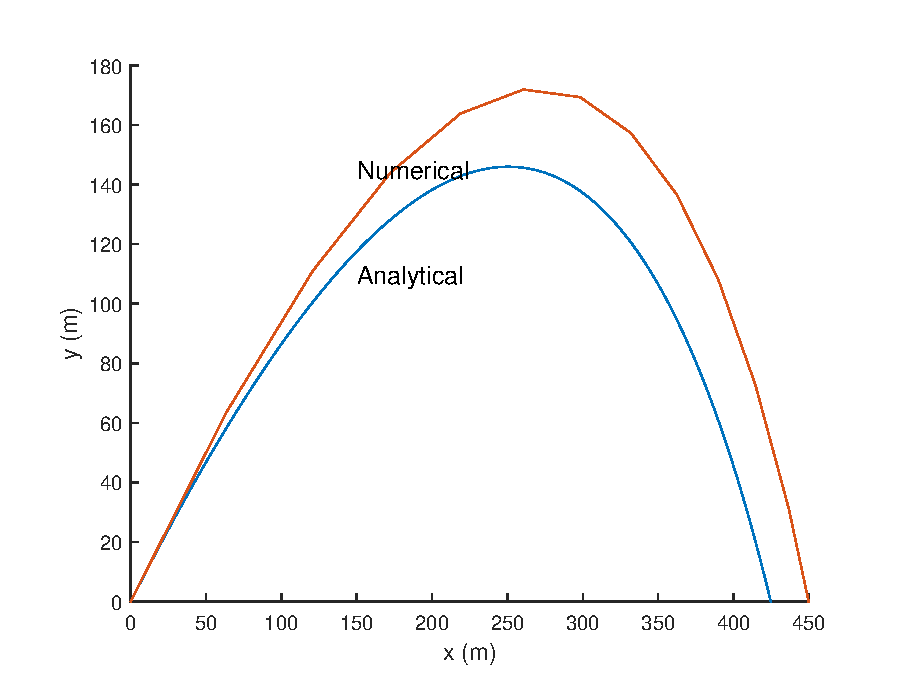
\includegraphics[height=5cm,width=10cm]{linear_figure2_1.eps}
\caption{Tragectories with $\Delta t=1s$} 
\end{figure}
\\When $\Delta t=0.5s$:
\begin{figure}[!htb] 
\centering 
\includegraphics[height=5cm,width=10cm]{linear_figure2_2.eps}
\caption{Tragectories with $\Delta t=0.5s$} 
\end{figure}
\newpage
\noindent When $\Delta t=0.01s$:
\begin{figure}[!htb] 
\centering 
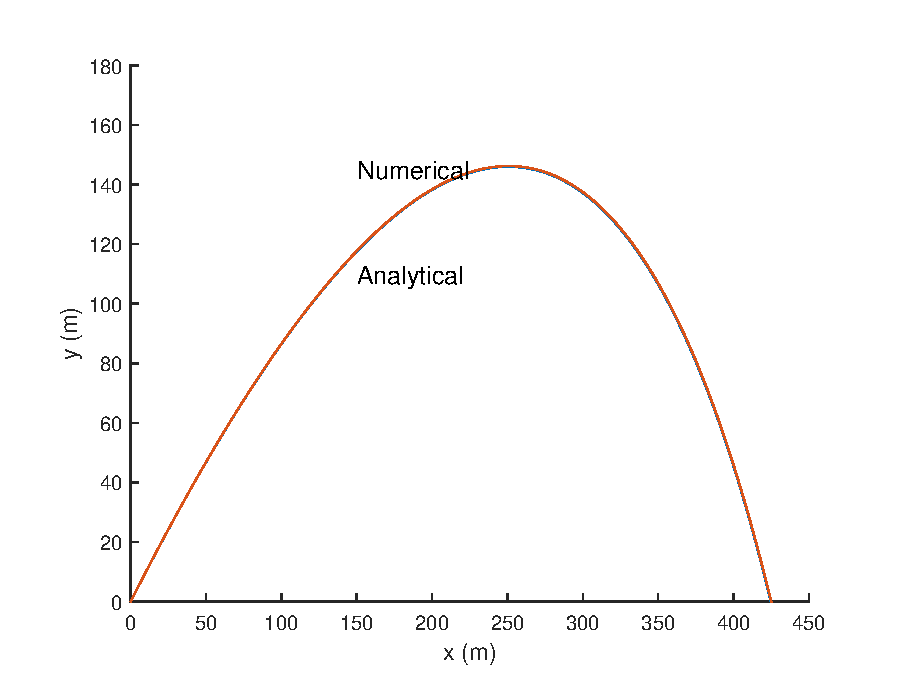
\includegraphics[height=5cm,width=10cm]{linear_figure2_3.eps}
\caption{Tragectories with $\Delta t=0.01s$} 
\end{figure}
\\The difference figure is:
\begin{figure}[!htb] 
\centering 
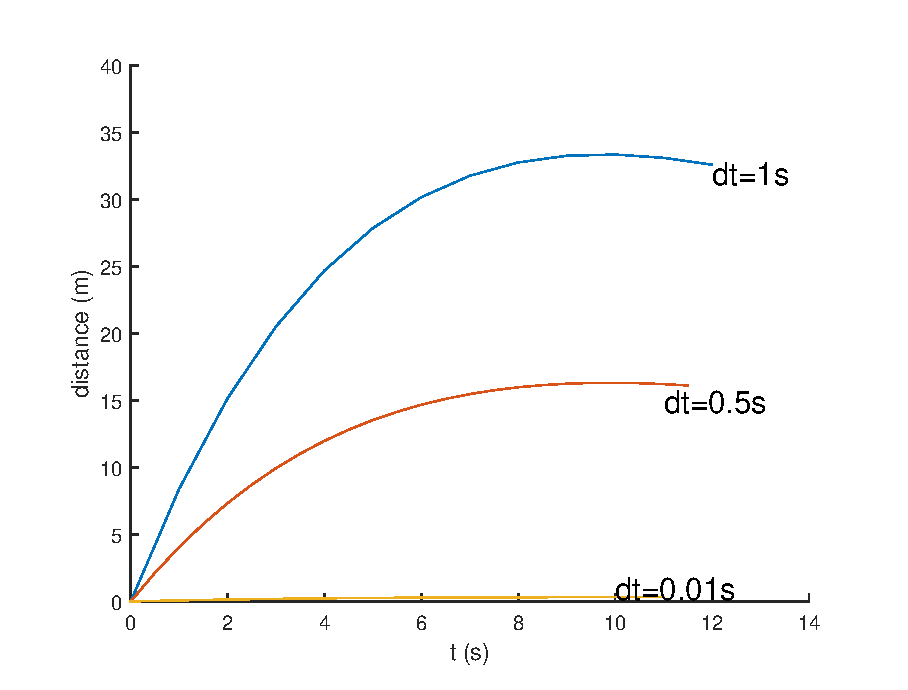
\includegraphics[height=5cm,width=10cm]{linear_figure2_4.eps}
\caption{Relationship between differences and time}
\end{figure}
\subsection{}
We choose $k=0.1$ and $\Delta t=0.01s$. Take $\alpha=\frac{\pi}{2},\frac{\pi}{3},\frac{\pi}{4},\frac{\pi}{5},\frac{\pi}{6}$
\subsubsection*{(a)}
\begin{figure}[!htb] 
\centering 
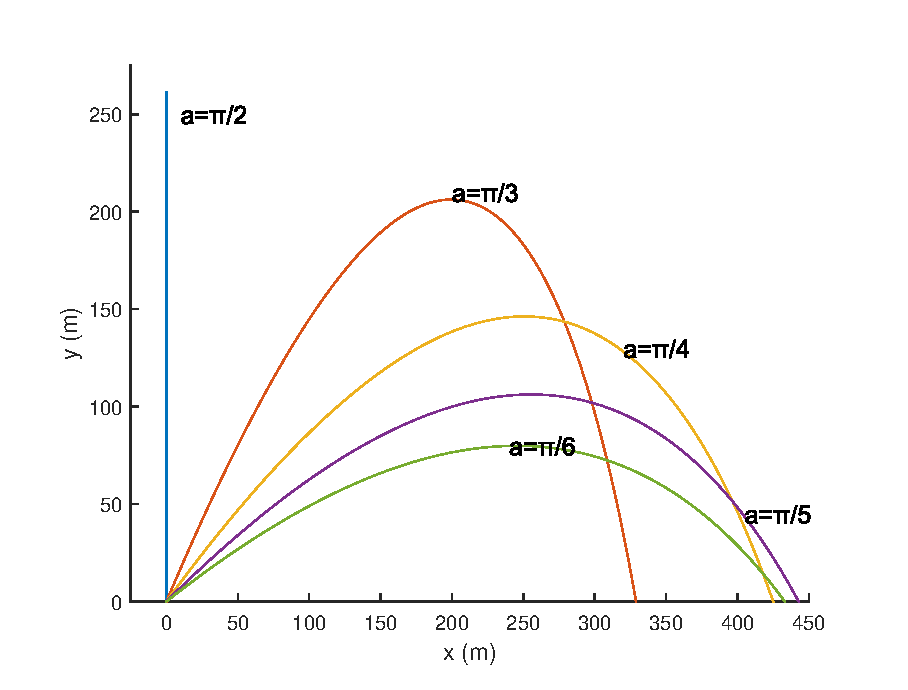
\includegraphics[height=4.5cm,width=8cm]{linear_figure3_1.eps}
\caption{Trajectories with different $\alpha$}
\end{figure}
\noindent As $\alpha$ increases, the highest point is higher and higher. When $\alpha=\frac{\pi}{2}$, it can reach the highest point; the range it reaches increases from 0 to certain point and then decreases. It no longer reaches the farthest point when $\alpha=\frac{\pi}{4}$.
\subsubsection*{(b)}
\begin{figure}[!htb] 
\centering 
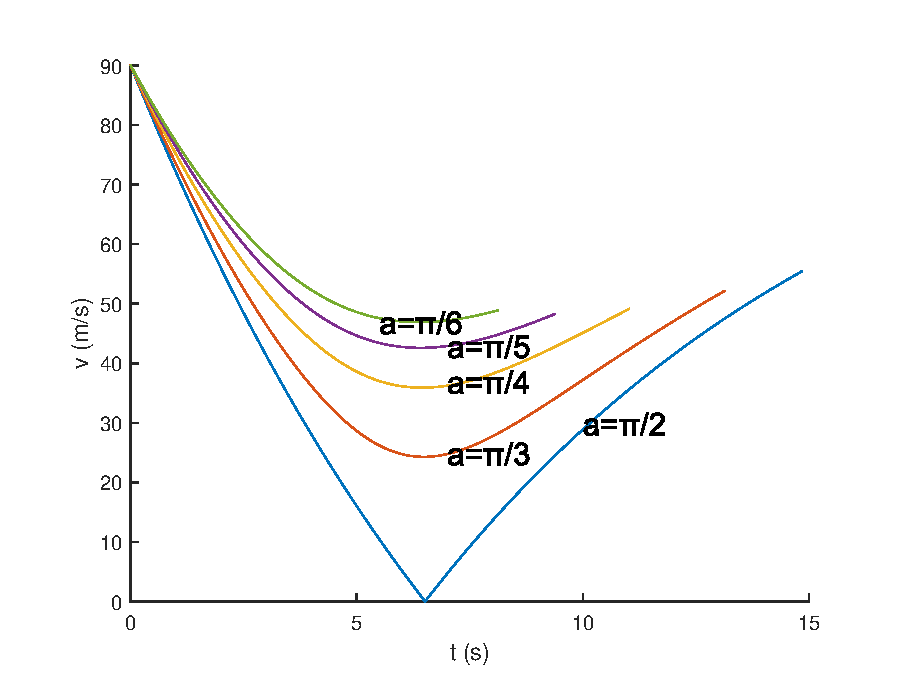
\includegraphics[height=5cm,width=10cm]{linear_figure3_2.eps}
\caption{Relationship between speed and time}
\end{figure}
\noindent We can conclude that:\\
1. The bigger $\alpha$, the longer time it keep in the air and the more rapid the speed change, the lower slowest speed it can achieve.\\
2. The speed-increasing rate is lower than speed-decreasing speed for same $\alpha$.\\
3. The terminal speeds are closed to each other.
\subsection{}
\noindent
We choose $\alpha=\frac{\pi}{4}$ and $\Delta t=0.01s$. Take k=0.02,0.05,0.1,0.2,0.5.
\subsubsection*{(a)}
\begin{figure}[!htb] 
\centering
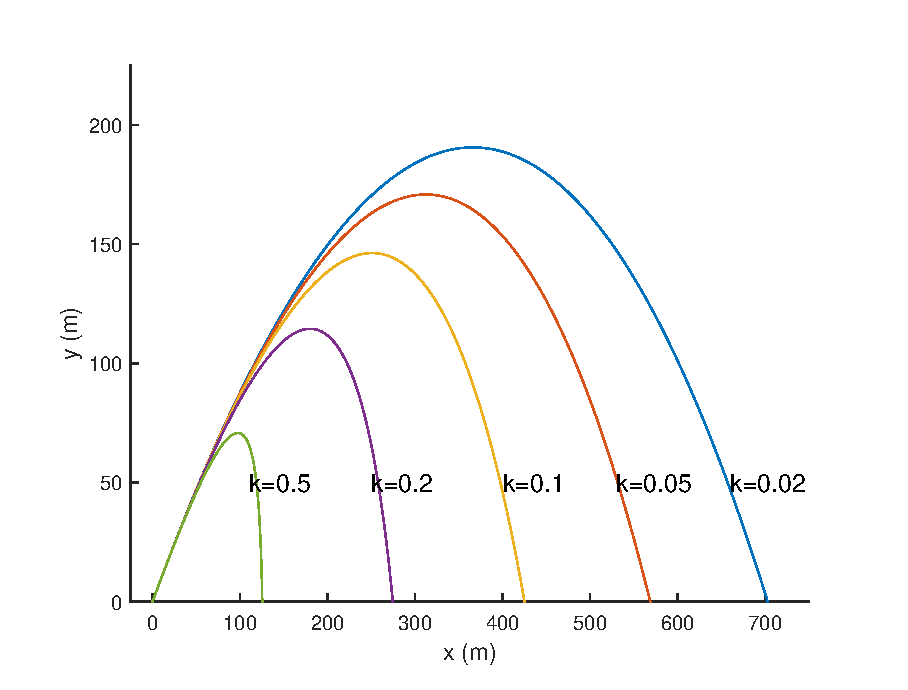
\includegraphics[height=5cm,width=10cm]{linear_figure4_1.eps}
\caption{Trajectories with different k($\kappa$)}
\end{figure}
\noindent As k is getting smaller, the range and maximum height is getting larger.
\newpage
\subsubsection*{(b)}
\begin{figure}[!htb] 
\centering 
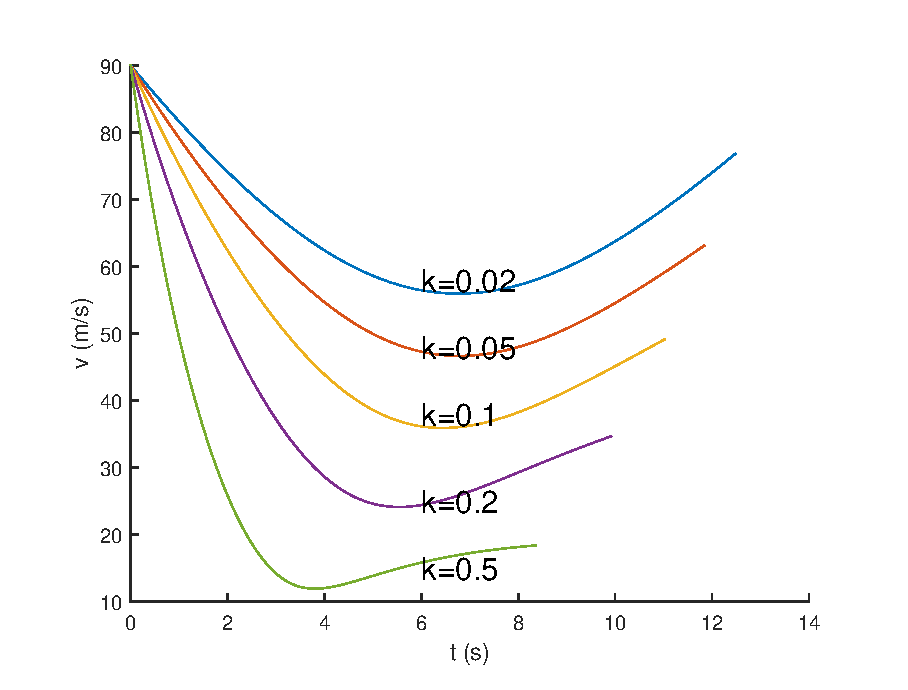
\includegraphics[height=5cm,width=10cm]{linear_figure4_2.eps}
\caption{Relationship between speed and time}
\end{figure}
\noindent As k is getting smaller:\\
1. The time it keeps in the air is longer.\\
2. The average speed is higher.\\
3. The rate of changing of the speed-decreasing is lower and that of speed-increasing is higher. \\
4. Overall kinetic energy loss is smaller.
\subsection{}
We can obviously get:
$$\begin{cases}
v_{x(i+1)}=v_{x(i)}-\frac{bv_iv_{x(i)}}{m}\Delta t\\
v_{y(i+1)}=v_{y(i)}-(g+\frac{bv_iv_{y(i)}}{m})\Delta t\\
t_{i+1}=i\Delta t
\end{cases}$$
and
$$\begin{cases}
x_{i+1}=x_i+v_{x(i)}\Delta t\\
y_{i+1}=y_i+v_{y(i)}\Delta t\\
t_{i+1}=i\Delta t
\end{cases}$$
\subsection{}
We set $b=0.001$ and $\alpha=\frac{\pi}{4}$.
\begin{figure}[!htb] 
\centering 
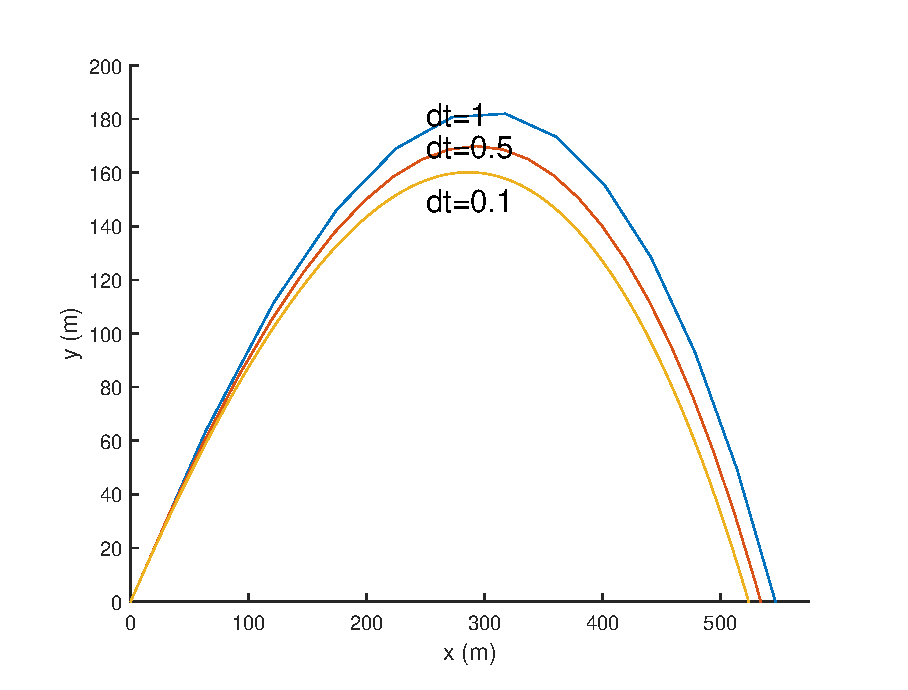
\includegraphics[height=5cm,width=10cm]{linear_figure6.eps}
\caption{Trajectories with different $\Delta t$}
\end{figure}
\\According to experience we had in previous problem, the more we divide the step, the more accurate it is. As the step becoming smaller, the "curve" is becoming smooth and the overall trajectory is lower.
\subsection{}
We choose $b=0.001$ and $\Delta t=0.1s$. Take $\alpha=\frac{\pi}{2},\frac{\pi}{3},\frac{\pi}{4},\frac{\pi}{5},\frac{\pi}{6}$
\subsubsection*{(a)}
\begin{figure}[!htb] 
\centering 
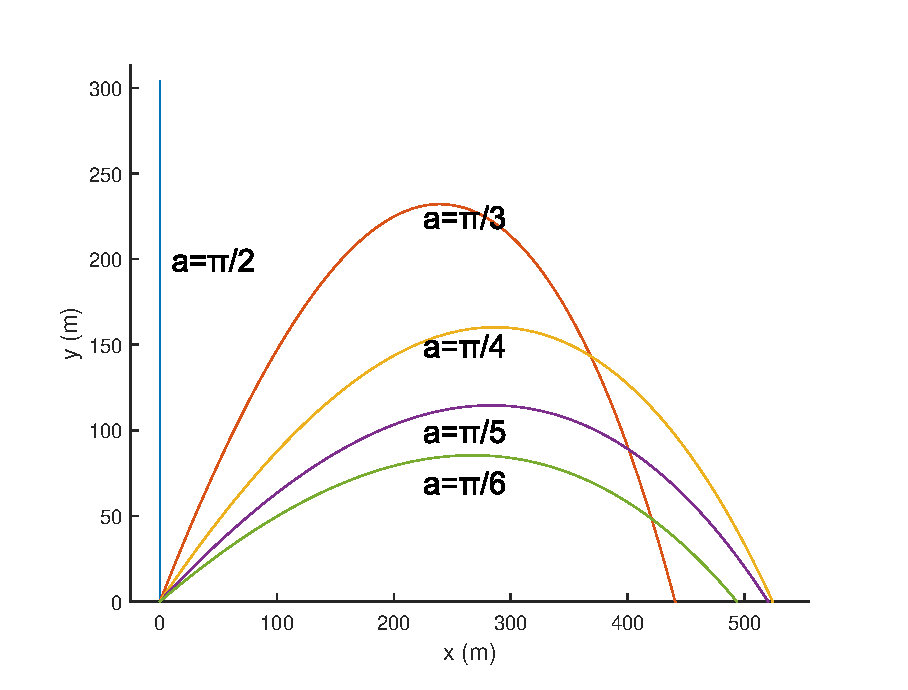
\includegraphics[height=5cm,width=10cm]{linear_figure7_1.eps}
\caption{Trajectories with different $\alpha$}
\end{figure}
As $\alpha$ increases, the highest point is higher and higher. When $\alpha=\frac{\pi}{2}$, it can reach the highest point; the range it reaches increases from 0 to certain point and then decreases.
\subsubsection*{(b)}
\begin{figure}[!htb] 
\centering 
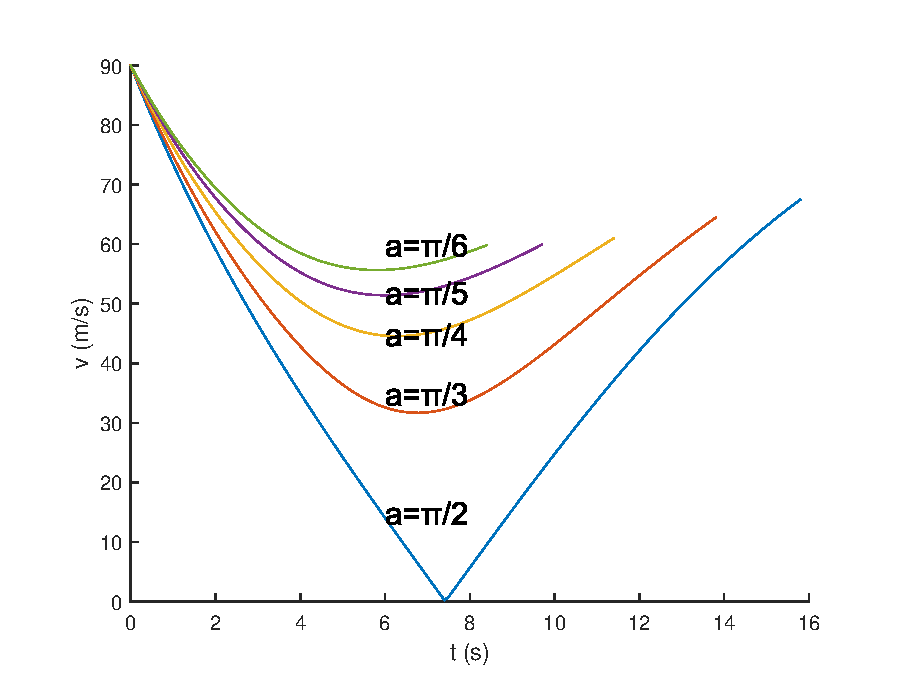
\includegraphics[height=5cm,width=10cm]{linear_figure7_2.eps}
\caption{Relationship between speed and time}
\end{figure}
\noindent We can conclude that:\\
1. The bigger $\alpha$, the longer time it keep in the air and the more rapid the speed change, the lower slowest speed it can achieve.\\
2. The speed-increasing rate is lower than speed-decreasing speed for same $\alpha$.\\
3. The terminal speeds are closed to each other.
\newpage
\subsection{}
We choose $\alpha=\frac{\pi}{4}$ and $\Delta t=0.1s$. Take $b=0.0002,0.0005,0.001,0.002,0.005$
\subsubsection*{(a)}
\begin{figure}[!htb] 
\centering 
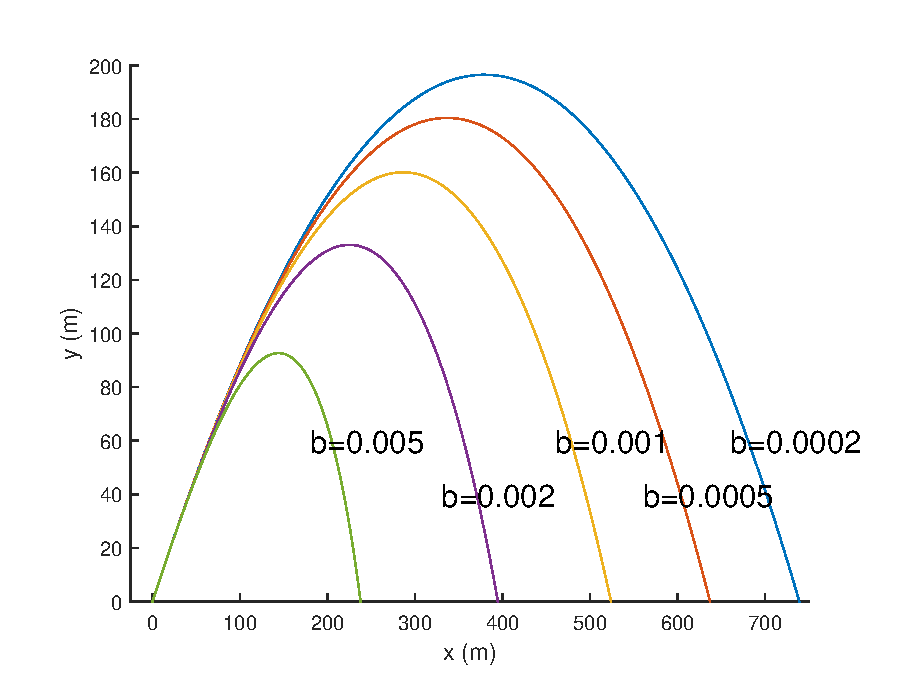
\includegraphics[height=5cm,width=10cm]{linear_figure8_1.eps}
\caption{Trajectories with different b($\beta$)}
\end{figure}
As b is getting smaller, the range and maximum height is getting larger.
\subsubsection*{(b)}
\begin{figure}[!htb] 
\centering 
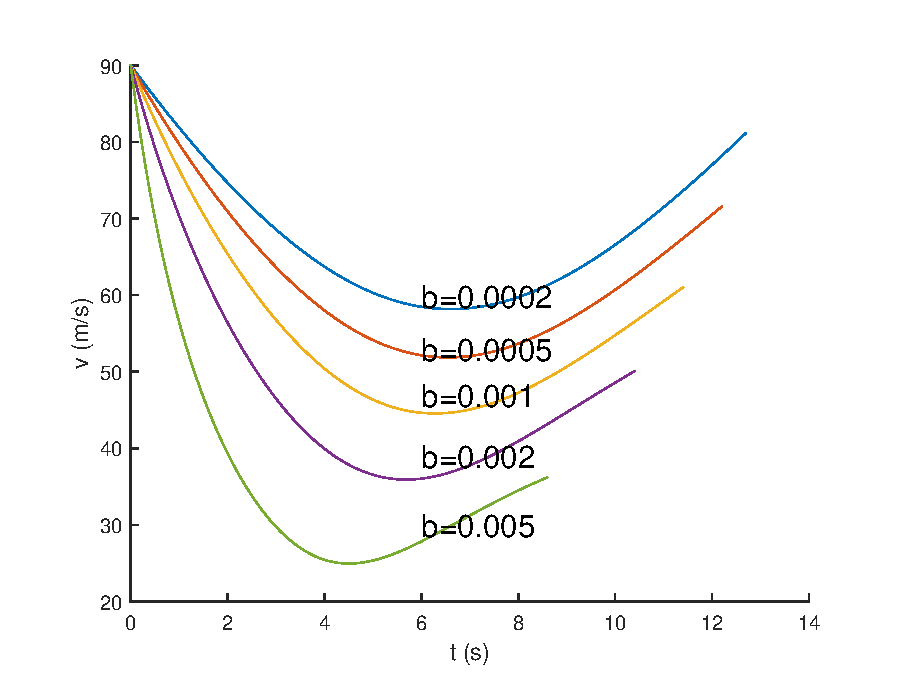
\includegraphics[height=5cm,width=10cm]{linear_figure8_2.eps}
\caption{Relationship between speed and time}
\end{figure}
\noindent As b is getting smaller:\\
1. The time it keeps in the air is longer.\\
2. The average speed is higher.\\
3. The rate of changing of the speed-decreasing is lower and that of speed-increasing is higher.\\
4. Overall kinetic energy loss is smaller.
\newpage
\subsection{}
Since the terminal speeds of linear and quadratic drag are the same, we can yield $kv=bv^2=mg$. let k=0.1, we can yield that $b=\frac{k^2}{mg}=\frac{1}{980}$.
\begin{figure}[!htb] 
\centering 
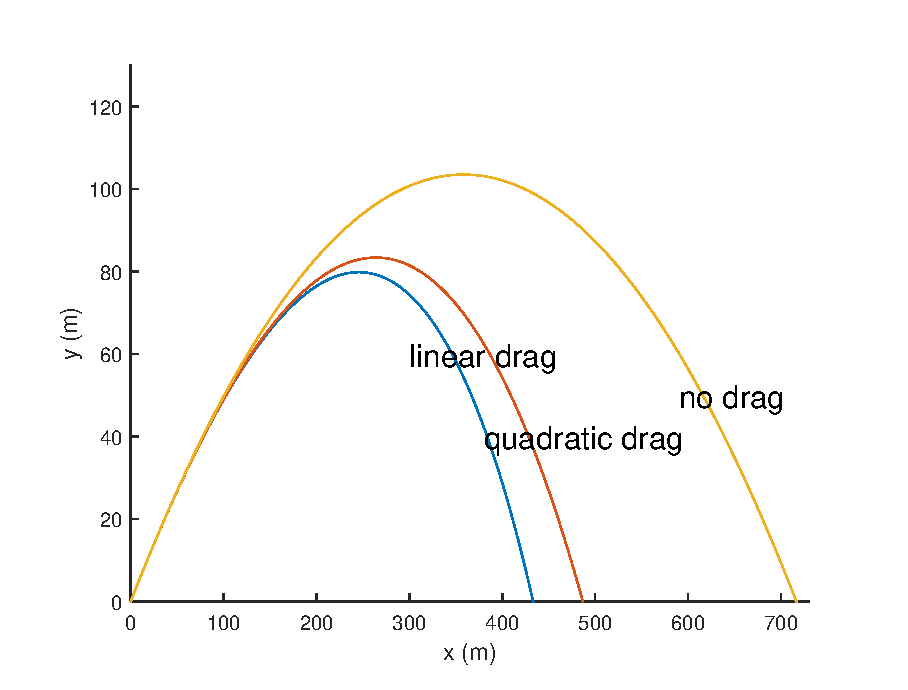
\includegraphics[height=5cm,width=10cm]{linear_figure9.eps}
\caption{Trajectories with different non-drag, linear-drag and quadratic-drag}
\end{figure}
\noindent \\As the order of velocity gets higher in the drag, the maximum height, the maximum range become smaller.
\section{Simple harmonic oscillator}
\subsection{}
According to Euler Method:
\begin{eqnarray*}
	f_{i+1} & = & f_{i}+G(f_i,t_i) \Delta t\\
	v_x& =& G(x,t)\\
	a_x& =& G(v,t)
\end{eqnarray*}
Hence we can easily yield that recursive equation of the velocity and position of oscillating paticle in 1D should be:\\
\begin{eqnarray*}
	v_{x,i+1}&=& v_{x,i}-\omega_0^2x_i\Delta t=v_{x,i}-\frac{9}{4}x_i\Delta t\\
	x_{i+1}&=& x_i+v_{x,i}\Delta t\\
	t_{i+1}&=& i\Delta t
\end{eqnarray*}
\\
\subsection{}
Since the acceleration is proportional to the displacement, the oscillation is harmonic. Thus we let: 
$$x=A\cos(\omega t+\varphi).$$
Thus $\forall t\ge0$:
$$-A\omega^2\cos(\omega t+\varphi)=-\omega_0^2A\cos(\omega t+\varphi)\quad\Rightarrow\quad \omega=\omega_0.$$
And since $x(0)=0.5$, $v_{x}(0)=1$, $\omega_0=1.5$, we get:
$$\left\{\begin{array}{l}
A\cos(\varphi)=\frac{1}{2}\\
-A\frac{3}{2}\sin(\varphi)=1
\end{array}\right. \quad\Rightarrow\quad \left\{\begin{array}{l}
A=\frac{5}{6}\\
\varphi=-\arctan\frac{4}{3}
\end{array}\right..$$
Thus the equation in the configuration space is :
$$x=\frac{5}{6}\cos(\frac{3}{2}t-\arctan\frac{4}{3}).$$
\\
\\Moreover, we have known:
\begin{eqnarray*}
	\frac{dv_x}{dt}&=&-\omega_0^2x \\
	\frac{dx}{dt}&=& v_x
\end{eqnarray*}
Divide them and get:
$$\frac{dv_x}{dx}=-\omega_0^2\frac{x}{v_x}\quad \Rightarrow \quad v_xdv_x+\omega_0^2xdx=0\quad \Rightarrow \quad \int v_xdv_x+\int\omega_0^2xdx=0 \quad \Rightarrow \quad v_x^2+\omega_0^2x^2=c,\;\textrm{where } c \textrm{ is constant}$$
Now we get:
$$\frac{v_x^2}{c}+\frac{\omega_0^2x^2}{c}=1.$$
And since $x(0)=0.5$, $v_{x}(0)=1$, $\omega_0=1.5$, we get:
$$\frac{1}{c}+\frac{9}{16c}=1 \quad \Rightarrow \quad c=\frac{25}{16}.$$
Thus the equation in the phase space is :
$$\frac{16v_x^2}{25}+\frac{36x^2}{25}=1.$$
\\Now we use matlab to draw the plots:
\\When $\Delta t=0.1s$ :
\begin{figure}[!htb]
	\begin{center}
		\includegraphics[height=5cm,width=10cm]{Problem2_1configuration}
	\end{center}
	\caption{numerical and analytical result in configuration space with $\Delta t=0.1s$}
\end{figure}
\newpage
\begin{figure}[!htb]
	\begin{center}
		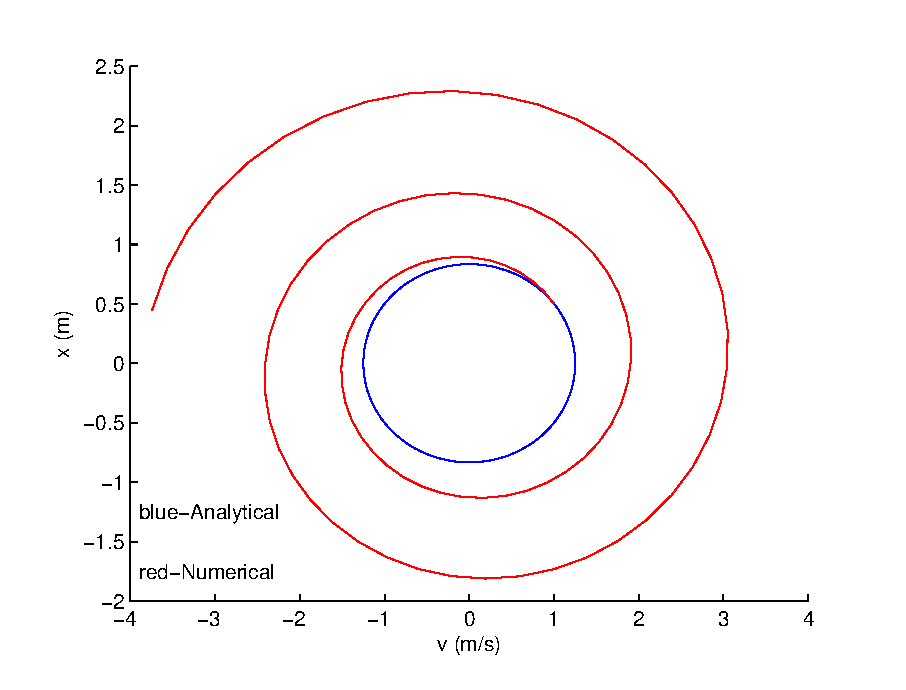
\includegraphics[height=5cm,width=10cm]{Problem2_1phase}
	\end{center}
	\caption{numerical and analytical result in phase space with $\Delta t=0.1s$}
\end{figure}
\noindent When $\Delta t=0.01s$ :
\begin{figure}[!htb]
	\begin{center}
		\includegraphics[height=5cm,width=10cm]{Problem2_2configuration}
	\end{center}
	\caption{numerical and analytical result in configuration space with $\Delta t=0.01s$}
\end{figure}
\begin{figure}[!htb]
	\begin{center}
		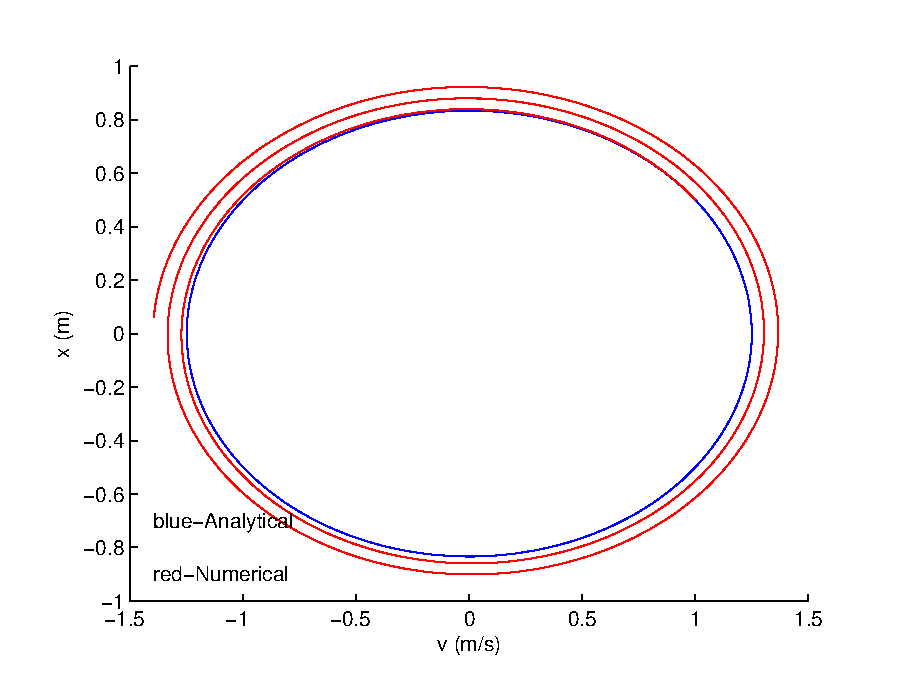
\includegraphics[height=5cm,width=10cm]{Problem2_2phase}
	\end{center}
	\caption{numerical and analytical result in phase space with $\Delta t=0.01s$}
\end{figure}
\newpage
\noindent When $\Delta t=0.001s$ :
\begin{figure}[!htb]
	\begin{center}
		\includegraphics[height=5cm,width=10cm]{Problem2_3configuration}
	\end{center}
	\caption{numerical and analytical result in configuration space with $\Delta t=0.001s$}
\end{figure}
\begin{figure}[!htb]
	\begin{center}
		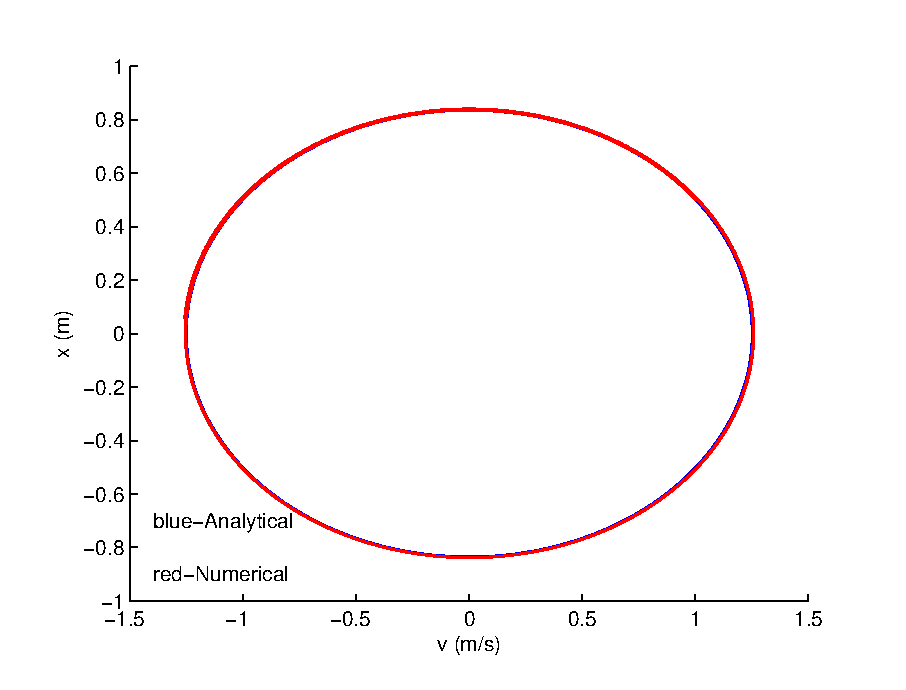
\includegraphics[height=5cm,width=10cm]{Problem2_3phase}
	\end{center}
	\caption{numerical and analytical result in phase space with $\Delta t=0.001s$}
\end{figure}
\\The difference figure in configuration space is :
\begin{figure}[!htb]
	\begin{center}
		\includegraphics[height=5cm,width=10cm]{Problem2differenceconfiguration}
	\end{center}
	\caption{difference between numerical and analytical result in configuration space}
\end{figure}
\subsection{}
Let $m=1kg$, $\Delta t=0.001s $ and use matlab to get the figure of $E(t)$:
\begin{figure}[!htb]
	\begin{center}
		\includegraphics[height=5cm,width=10cm]{Problem3}
	\end{center}
	\caption{total energy $E(t)$ in Euler and analytical cwith $\Delta t=0.001s$ and $m=1kg$}
\end{figure}
\\\indent The numerical $E(t)$ is close to the analytical $E(t)$, but we can obviously see that the numerical $E(t)$ has an angle of slope, which makes the difference between numerical result and analyitical one greater when $t$ is greater. And we should also notice that $\Delta t=0.001s$ is small enough to make the difference between $x$ and $t$ seem like horizontial in the Figure 21. The possible reason of the appearance of the obvious error may be $E(t)$ includes a square of $x$ and $v_x$, and the errors in $x$ and $v$ become greater.
\\\indent Anyway, if we take smaller $\Delta t$, we can get a $E(t)$ more horizontial. Approximately, we can regard the value of $E(t)$ as a constant. The physical meaning here is that the total energy of the harmonic osillcation is constant, since $\frac{1}{2}m\omega_0^2x^2$ is the elastic potential energy, and $\frac{1}{2}nv_x^2$ is the kinetic energy.
\subsection{}
According to Runge-Kutta Method:
\begin{eqnarray*}
	f_{i+1} & = & f_{i}+G(f_i+\frac{G(f_i,t_i)\Delta t}{2},t_i+\frac{\Delta t}{2}) \Delta t\\
\mathbf{v} & = & G(\mathbf{x},t)\\
\mathbf{a} & = & G(\mathbf{v},t)
\end{eqnarray*}
Hence we can easily yield that recursive equation of the velocity and position of oscillating paticle in 1D should be:\\
\begin{eqnarray*}
	x(t_{i+1})&=& x(t_i)+v(t_i+\frac{\Delta t}{2})\Delta t\\
	v(t_i+\frac{\Delta t}{2})&=& v(t_i)-\omega_0^2x_i\frac{\Delta t}{2}\\
	t_{i+1}&=& i\Delta t
\end{eqnarray*}
Then we get:
\begin{eqnarray*}
	x_{i+1}&=& x_{i}+v_{i}\Delta t-\omega_0^2x_i\frac{\Delta t^2}{2}=x_{i}+v_{i}\Delta t-\frac{9}{8}x_i\Delta t^2\\
	v_{i+1}&=& v_i-\omega_o^2x_i\Delta t-\omega_0^2v_i\frac{\Delta t^2}{2}=v_i-\frac{9}{4}x_i\Delta t-\frac{9}{8}v_i\Delta t^2\\
	t_{i+1}&=& i\Delta t
\end{eqnarray*}
\subsection{}
Use matlab and let $\Delta t=0.1s$, we get the figure in configuration space :
\begin{figure}[!htb]
	\begin{center}
		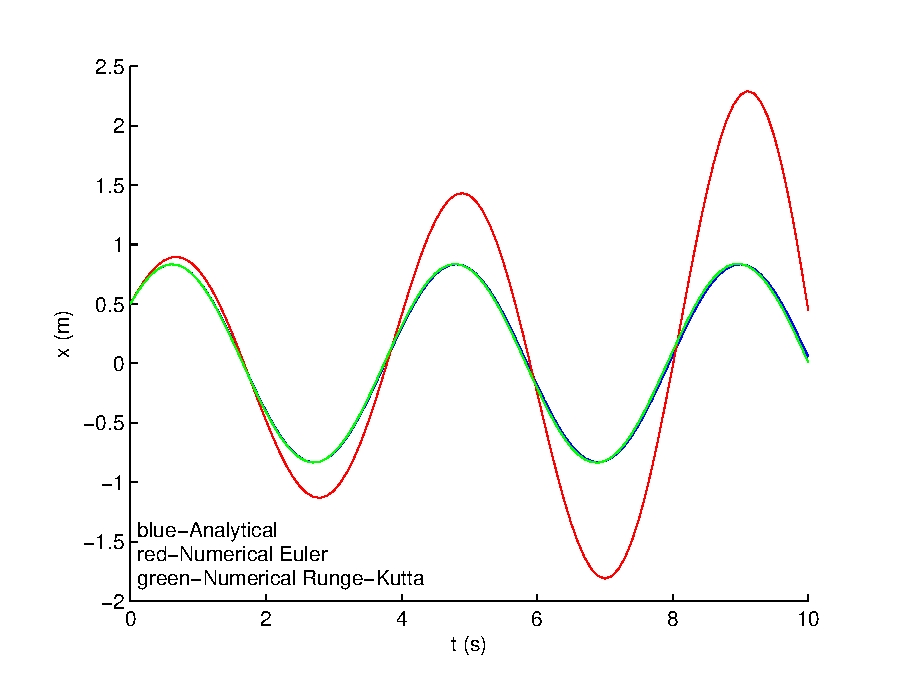
\includegraphics[height=4.5cm,width=7cm]{Problem5RKconfiguration}
	\end{center}
	\caption{Euler numerical, Runge-Kutta numerical and analytical result in configuration space}
\end{figure}
\\And in phase space:
\begin{figure}[!htb]
	\begin{center}
		\includegraphics[height=4.5cm,width=7cm]{Problem5RKphase}
	\end{center}
	\caption{Euler numerical, Runge-Kutta numerical and analytical result in phase space}
\end{figure}
\\\indent We can see that in either configuration or phase space, the trajectory producted by the Runge-Kutta method is very close to the analytical result, while the one producted by the Euler method has a obvious error. This fact shows that the Runger-Kutta method can get a more accurate numerical result than the Euler method.
\\Now we consider $E(t)$, when $\Delta t=0.1s$ and $m=1kg$ :
\begin{figure}[!htb]
	\begin{center}
		\includegraphics[height=4.5cm,width=7cm]{Problem5energy}
	\end{center}
	\caption{total energy $E(t)$ in Euler, Runger-Kutta and analytical with $\Delta t=0.1s$ and $m=1kg$}
\end{figure}
\\
\\\indent We can see that the line producted by the Runge-Kutta method is very close to the analytical result, while the one producted by the Euler method has a very large error. This factor shows that the Runger-Kutta method can get a more numerical result than the Euler method, and the accuracy of the energy can be largely improved if using the Runger-Kutta method instead of the Euler method.
\section{Remarks on the accuracy of numerical methods}
The accuracy of numerical methods can be improved by 2 ways.
\subsection{Reduce the time step}
For both Euler method and Second-order Runge-Kutta method, the smaller the time step is, the more accuracy the numerical solution is.
\begin{figure}[!htb]
	\begin{center}
		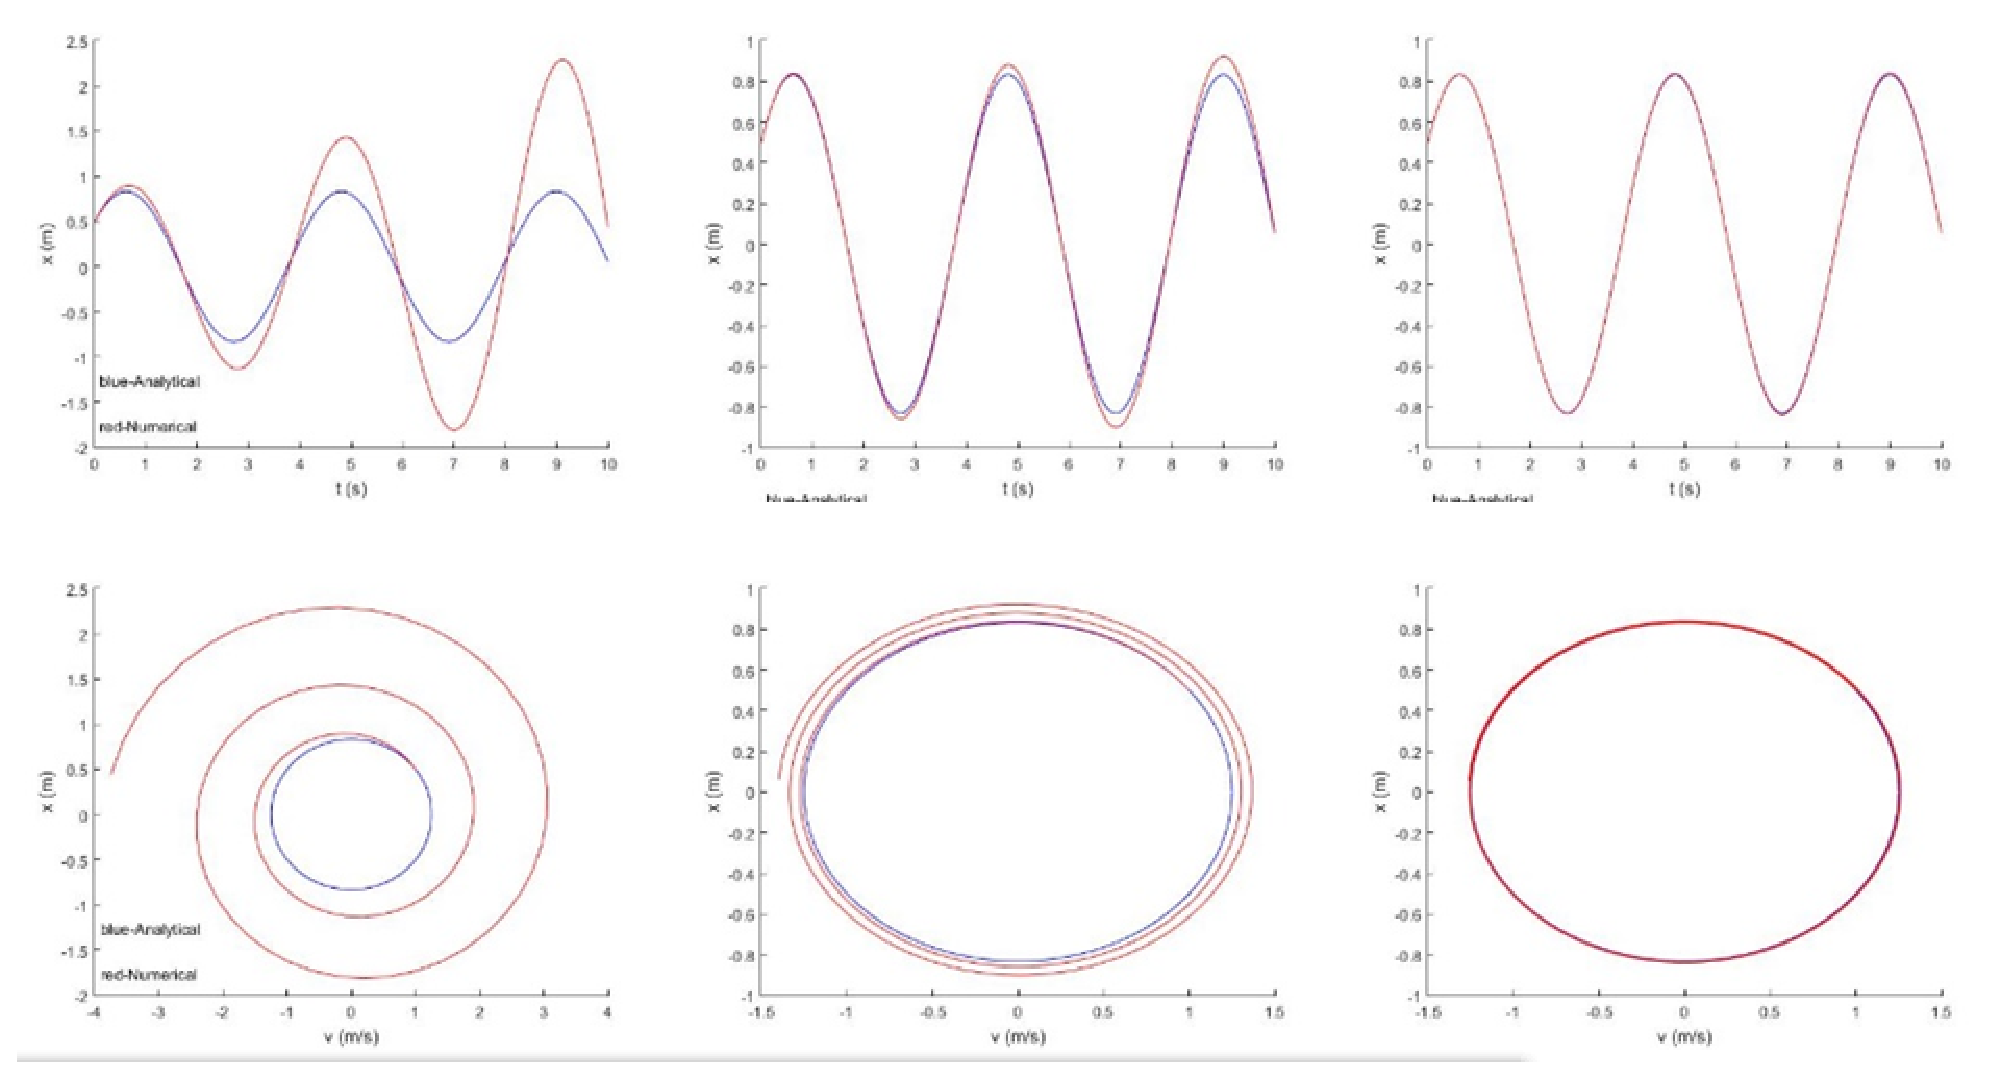
\includegraphics[height=5cm,width=10cm]{Section4}
	\end{center}
	\caption{Comparison between different $\Delta t$ in Euler method}
\end{figure}
\\Above pictures are numerical solutions (Red) compared with analytical solutions (Blue) by Euler method of time step $\Delta t=0.1s,\;0.01s,\;0.001s.$
\newpage
\begin{figure}[!htb]
	\begin{center}
		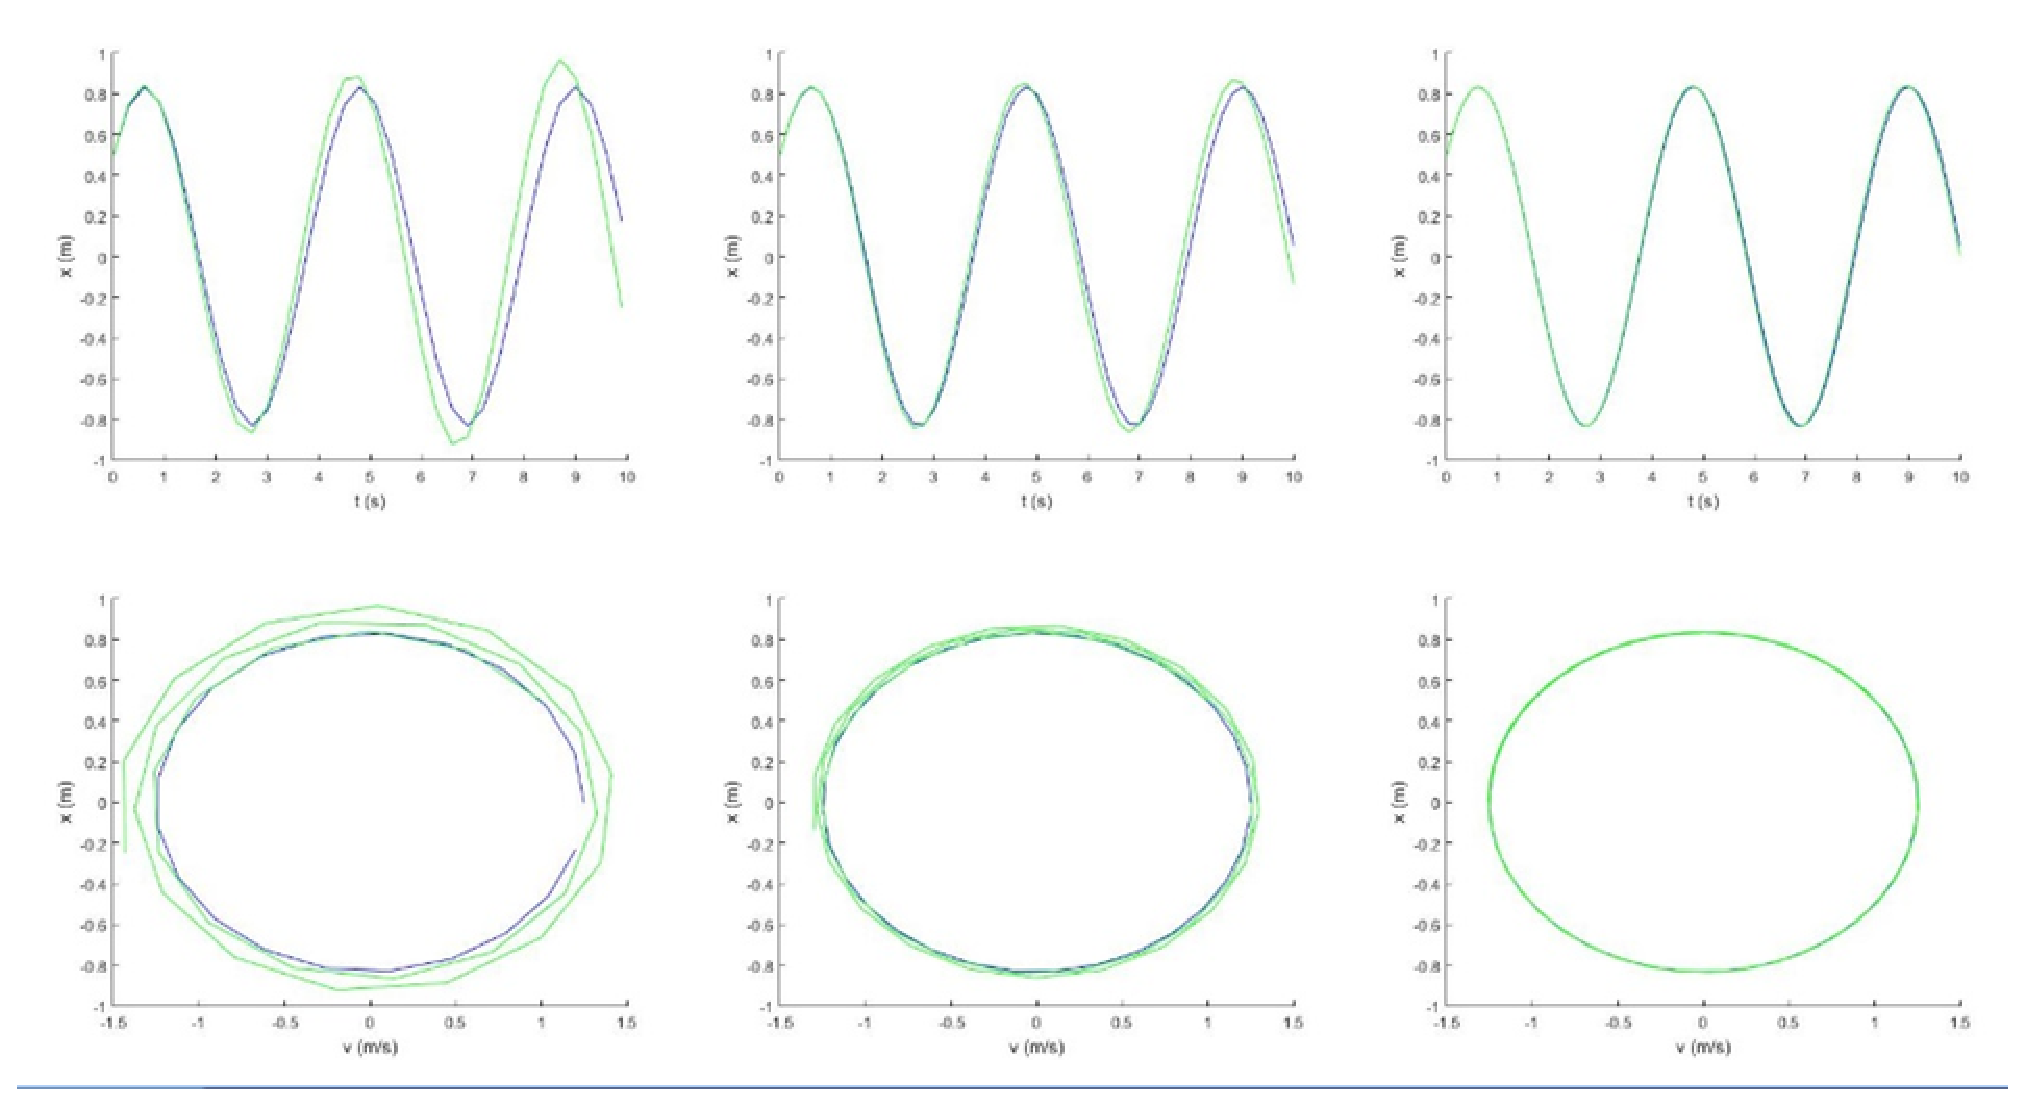
\includegraphics[height=5cm,width=10cm]{Section4_2}
	\end{center}
	\caption{Comparison between different $\Delta t$ in Rung-Kutta method}
\end{figure}
\noindent Above pictures are numerical solutions (Green) compared with analytical solutions (Blue) by Euler method of time step $\Delta t=0.3s,\;0.2s,\;0.1s.$
\\It is obviously according to the graphs that the accuracy of both methods increases when the time step reduce.
\subsection{Use more sophisticated algorithms}
Euler method is a kind of First-order Runge-Kutta method. Runge-Kutta becomes more accurate when the order rise.
\begin{figure}[!htb]
	\begin{center}
		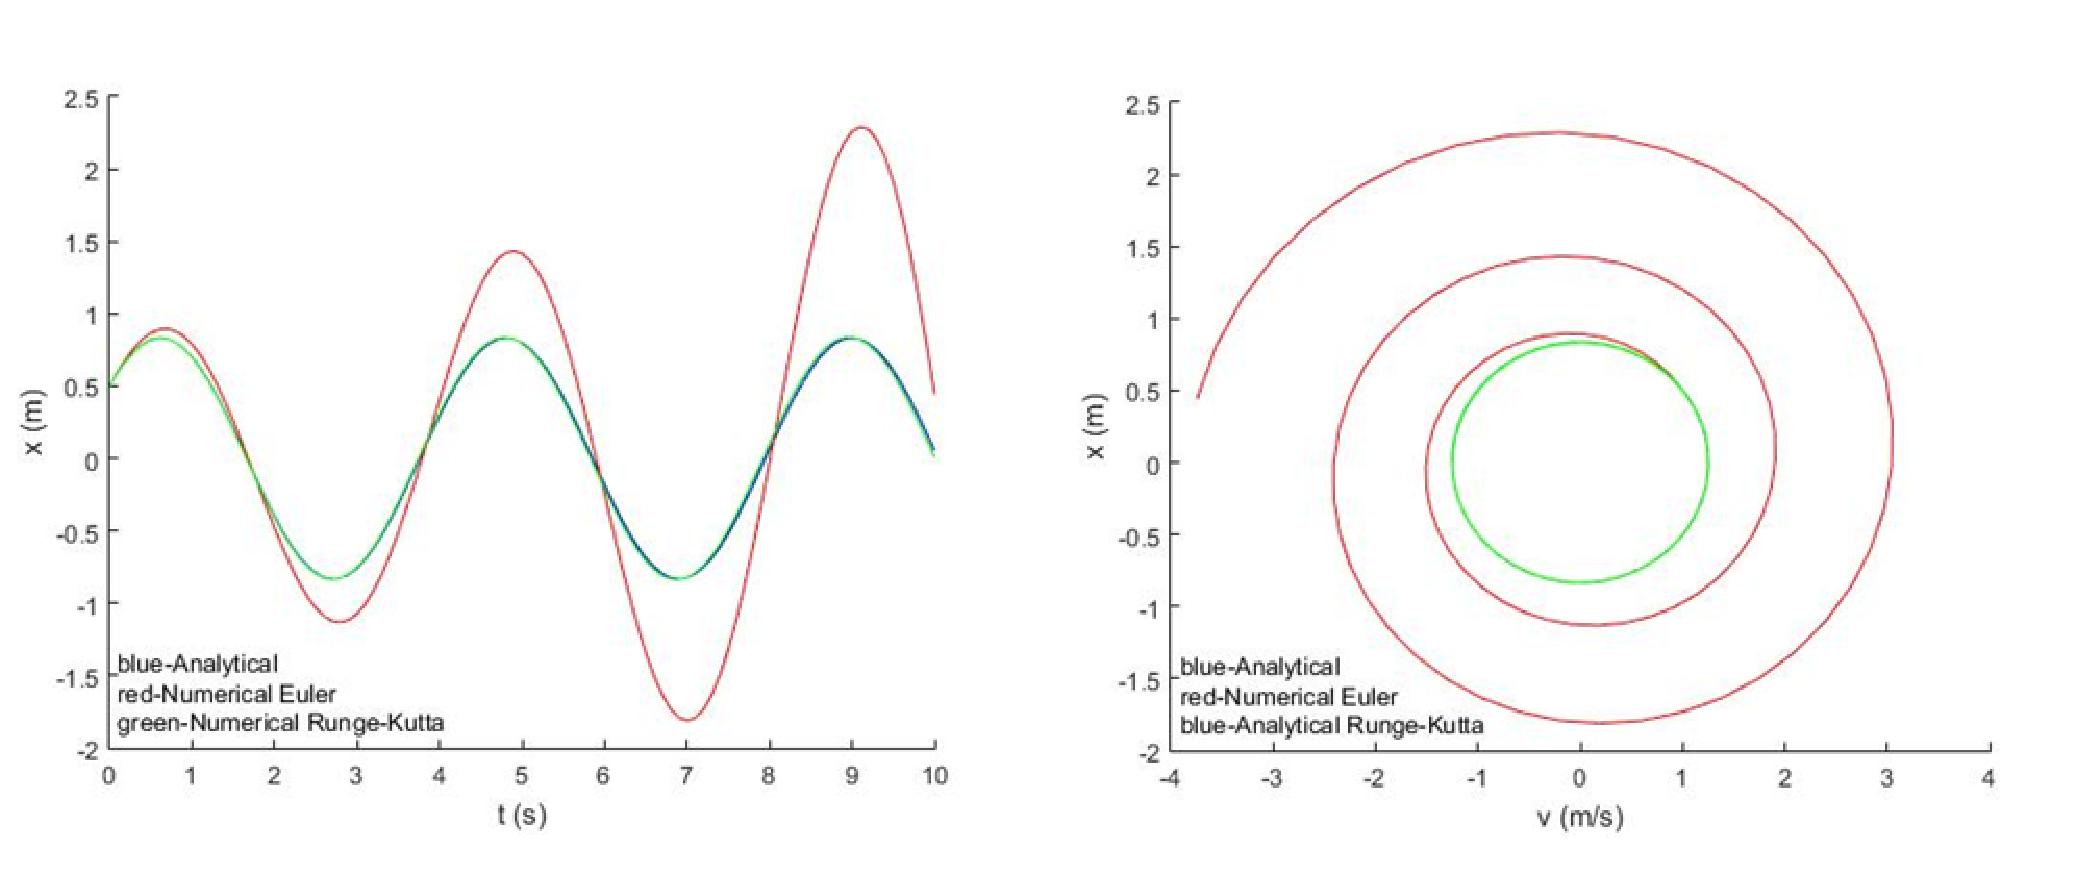
\includegraphics[height=5cm,width=10cm]{Section4_3}
	\end{center}
	\caption{Comparison between Euler method and Rung-Kutta method with $\Delta t=0.1s$}
\end{figure}
\\Above pictures are Euler numerical solutions (Red), Second-order Runge-Kutta numerical solutions (Green) compared with analytical solutions (Blue) by Euler method of time step $\Delta t=0.1s.$
\\It can be seen that Second-order Runge-Kutta is more accurate than Euler numerical solution for the same time step.
\\There are also some other methods that provides more accurate numerical solutions.
\\Function “NDSolveValue” in Mathematica provides more accurate numerical solution than Second-order Runge-Kutta method.
\begin{figure}[!htb]
	\begin{center}
		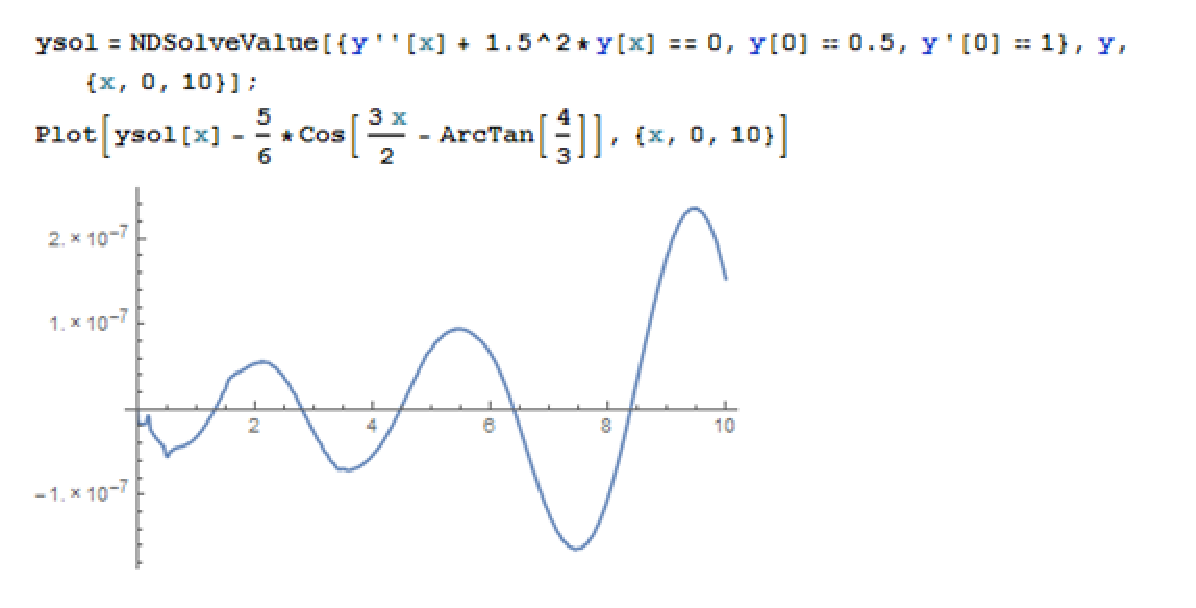
\includegraphics[height=5cm,width=10cm]{Section4_4}
	\end{center}
	\caption{differece between "NDSoluveValue" numerical result and analytical result}
\end{figure}
\\The picture above shows the accuracy of numerical solution provided by “NDSolveValue”.
\section{Optional Question}
By Second-order Runge-Kutta method:
\begin{eqnarray*}
f_{i+1}&=& f_{i}+G(f_i+\frac{G(f_i,t_i)}{2},t_i+\frac{\Delta t}{2})\Delta t\\
G_{f,t}&=& \frac{df}{dt}\\
t_{i+1}&=& i\Delta t
\end{eqnarray*}
Thus:
$$f(t_{i}+\Delta t)=f_{i+1}=f(t_{i})+f^{'}(t_i+\frac{\Delta t}{2})\Delta t.$$
By Taylor expansion:
$$f^{'}(t_i+\frac{\Delta t}{2})=f^{'}(t_i)+f^{''}(t_i)\frac{\Delta t}{2}+o(\Delta t).$$
Thus:
$$f(t_{i}+\Delta t)=f(t_{i})+f^{'}(t_i)\Delta t+f^{''}(t_i)\frac{\Delta t^2}{2}+o(\Delta t^2)=f(t_{i})+f^{'}(t_i)\Delta t+O(\Delta t^2).$$
Thus we conclude that $f$ is accurate to second order.
\\This means that the Second-order Runge-Kutta method is second order.
\\Next we will prove that the Eular method is first order.
By Eular method:
\begin{eqnarray*}
f_{i+1}&=& f_{i}+G(f_i,t_i)\Delta t\\
G(f,t)&=& \frac{df}{dt}\\
t_{i+1}&=& i\Delta t
\end{eqnarray*}
Thus we get:
$$f_{t_i+\Delta t}=f_{i+1}=f_(t_{i})+f^{'}(t_{i})\Delta t=f_(t_{i})+O(\Delta t).$$
Thus we conclude that $f$ is accurate to first order $\Delta t$.
\\This means that the Euler method is first order.
\section{Conclusion}
$\indent$In the first part of the project, we use Euler Algorithm to simulate the projectile motion with air drag. We see the power of Euler's algorithm and uses this method to discuss the effect of variables to the trajectory.\\
\indent In the second part of the project, we firstly use Euler Algorithm to simulate the 1D simple harmonic oscillation in both configuration and phase space. In both space we can see when $\Delta t$ is small enough, the numerical tarjectory is very close to the analytical tarjectory.And secondly we use Second-order Runge-Kutta method to simulate the oscillation in both space again. By comparing the result producted by the Euler method and the Second-order Runge-Kutta method, we conclude that the Second-order Runge-Kutta method can get a more accurate result, and the improvement of accuracy is very obvious when we simulate the total energy of the osillation.\\
\indent In the third part of the project, we check two factors that can affect the accuracy of the approximation by comparing the whole result we have got in the preivous parts of the project. And we conclude that reducing the time step and using more sophisticated algorithms can improve the accuracy of the approximation.\\
\indent In the forth part of the project, we use mathematical method such as Taylor expansion to prove Euler method is first order, and Second-order Runge-Kutta is actually second order.\\
\indent Through this project, we learn a lot about the idea of fitting to solve the difficult equations. Firstly, we learn two important idea/method to calculate the numerical solution. Secondly, we gain idea of numerical solution to get the data that is really needed for production. We also learn how to make our solution close to the analytical solution and combine our knowledge on programming to some practical issue. What's more, we develop our ability of cooperation in this process.
\end{document}